% Provenance (never printed): see sources/outline_sources.md (Year 1: continental
% rifting and break-up; passive-margin structure; fast and slow ridges; the depth--age
% law of the ocean floor; transform faults). Curve from figdata/bachelor-1/depth_age.py;
% exercise and problem values in the Book 3 scratch calculator calc/ch13.py; the
% coordinates of the margin schematic from calc/fig13_margin.py.
\chapter{Slenken, ruggen en passieve randen}\label{ch:b1:rifts-ridges-margins}

In september 2005 brak de grond van de Afar-woestijn, in het noordoosten van Ethiopië, open. Binnen drie weken werd een stuk van de \omterm{def:b1:rifts-ridges-margins:rift}{slenk}, ongeveer \qty{60}{km} lang, tot \qty{8}{m} breder, en steeg van onderaf ongeveer \qty{2.5}{km^3} magma de scheur in. De platen scheiden daar met ongeveer \qty{18}{mm} per jaar: de crisis gaf in enkele weken de rek vrij van ongeveer vierhonderd jaar. Afar is een continent dat uiteenvalt; enkele honderden kilometers noordelijker is de Rode Zee een jonge oceaan waarvan de bodem al is gemaakt zoals de bodem van de Atlantische Oceaan, en de Zuid-Atlantische Oceaan was zo'n \omterm{def:b1:rifts-ridges-margins:rift}{slenk} voordat zij openging, ongeveer 120 miljoen jaar geleden. Dit hoofdstuk volgt de geboorte van een oceaan: het uitrekken van een continent, zijn uiteenvallen, de twee \omterm{def:b1:rifts-ridges-margins:passive-margin}{passieve randen} die achterblijven, de rug die de oceaanbodem bouwt, en het langzame zinken van die bodem terwijl zij afkoelt.
% ledger: wright:afar, morvel:ar-nb (18.5 mm/yr at 12.3 N, 40.6 E, computed with euler_velocities.py), heine:fit

\begin{recall}
De platen vormen de bovenste \omterm{def:b1:heat-budget:boundary-layer}{thermische grenslaag} van de \omterm{def:b1:layered-earth:layers}{mantel}; onder de oceanen beschrijft een afkoelende halfruimte hen, en hun isothermen verdiepen zich als de vierkantswortel van de leeftijd (\cref{ch:b1:heat-budget}). Gesteenteskolommen in isostatisch evenwicht hebben dezelfde massa per oppervlakte-eenheid boven een \omterm{def:b1:isostasy-gravity:isostasy}{compensatiediepte} (\cref{ch:b1:isostasy-gravity}). Platen draaien om Eulerpolen, ruggen spreiden met snelheden die uit magnetische anomalieën worden afgelezen, en transforms liggen op \omterm{def:b1:spherical-astronomy:spherical-triangle}{kleine cirkels} rond de pool (\cref{ch:b1:plate-kinematics}). De \omterm{def:b1:cross-sections:throw}{worp} en de \omterm{def:b1:cross-sections:throw}{heave} van een breuk werden gedefinieerd in \cref{ch:b1:cross-sections}; een normale breuk is een schuine breuk waarvan het bovenste blok naar beneden is bewogen (Boek 2, klas 11).
\end{recall}

\section{Continentale riftvorming}

Een continent dat door krachten aan zijn randen wordt uitgerekt, dunt niet gelijkmatig uit. Zijn broze bovenkorst breekt langs normale breuken, en de blokken ertussen zakken en kantelen; daaronder stromen de warmere onderkorst en de \omterm{def:b1:layered-earth:layers}{mantel}.

\begin{definition}[Continentaal rift, slenk, halve slenk]\label{def:b1:rifts-ridges-margins:rift}
Een \emph{continentaal rift}\index{continentaal rift} is een lange, smalle zone waar een continent wordt uitgerekt: een depressie begrensd door normale breuken, met aardbevingen en, vaak, vulkanen. Een \emph{slenk}\index{slenk} is een blok dat tussen twee normale breuken naar beneden is gezakt, die naar elkaar toe hellen. Een \emph{halve slenk}\index{halve slenk} is een blok dat naar beneden is gezakt en tegen één grote normale breuk, de randbreuk, aan één kant is gekanteld.
\end{definition}

De meeste riftbekkens zijn ketens van \omterm{def:b1:rifts-ridges-margins:rift}{halve slenken}. Hun randbreuken geven de verplaatsing aan elkaar door via relaisrampen, en de kant van de randbreuk wisselt vaak van het ene segment naar het volgende. Het hangende blok van elke randbreuk kantelt naar haar toe, en het bekken vult zich daar het snelst: het dikste sediment stapelt zich op tegen de breuk, terwijl de liggende wand wordt opgetild tot de riftschouder.

De horizontale uitrekking die door een breuk wordt gedragen, is haar \omterm{def:b1:cross-sections:throw}{heave}. Een vlakke normale breuk met \omterm{def:b1:cross-sections:throw}{worp} $h$ en helling $\delta$ heeft de \omterm{def:b1:cross-sections:throw}{heave} $h/\tan\delta$ (\cref{ch:b1:cross-sections}); de \omterm{def:b1:cross-sections:throw}{heaves} van de breuken over een riftdoorsnede bij elkaar opgeteld geven de uitrekking van de broze \omterm{def:b1:layered-earth:layers}{korst}. Hoe de hele \omterm{def:b1:layered-earth:lithosphere}{lithosfeer} dunner wordt terwijl zij wordt uitgerekt, en waarom zij daarna zinkt, wordt gekwantificeerd in Boek 4; hier worden de breuken gemeten en hun som vergeleken met de beweging van de platen.

\begin{omfigure}
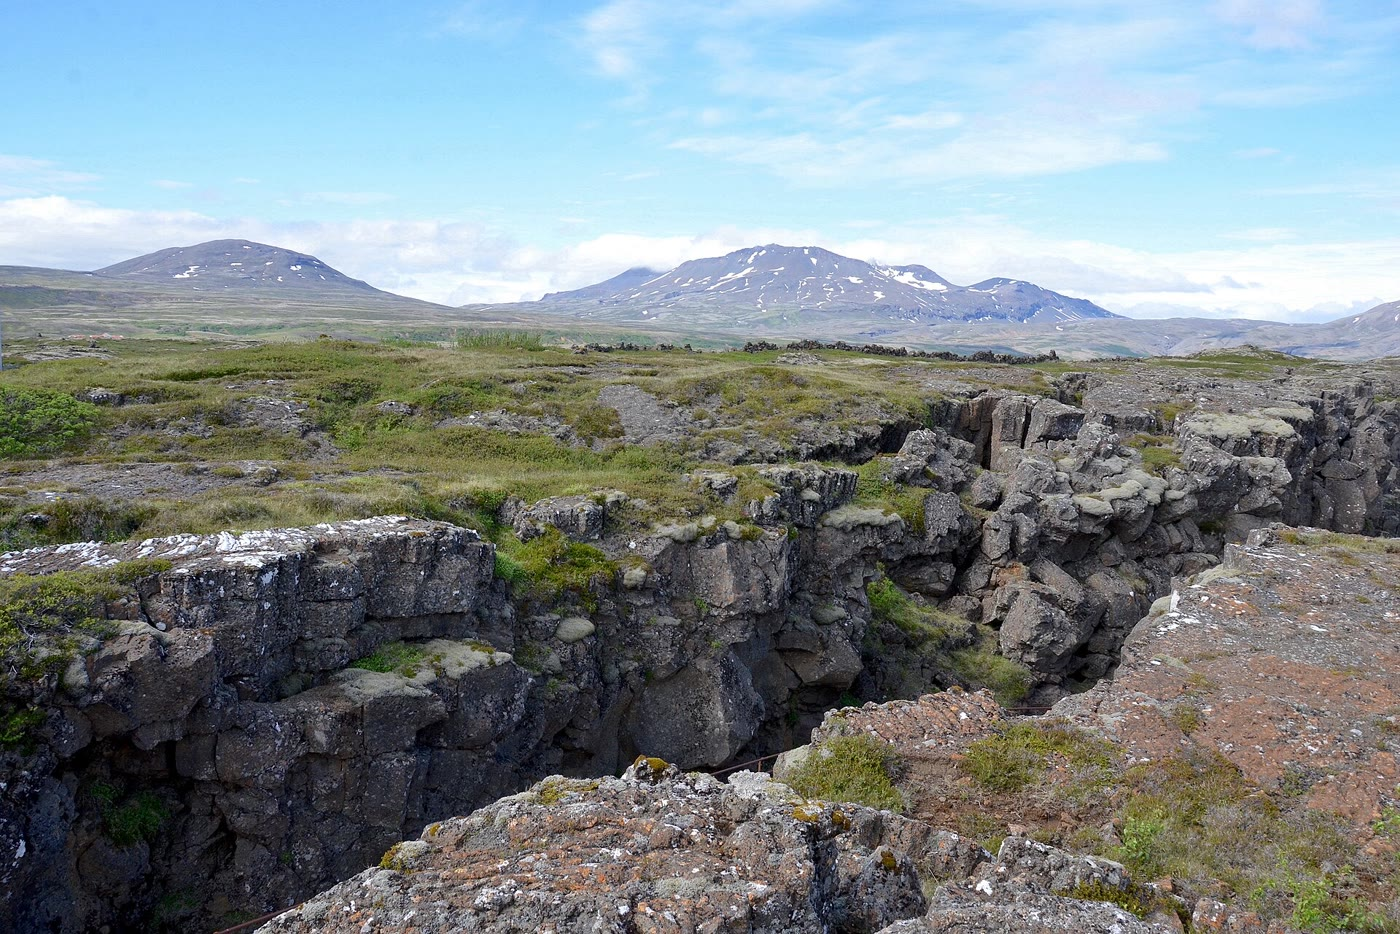
\includegraphics[width=0.8\linewidth]{images/book3/b1-thingvellir-fissure.jpg}

{\small Een open spleet in de lavavloer van het riftdal Þingvellir, in zuidwest-IJsland, waar de Mid-Atlantische Rug aan land komt. De basaltstromen van de dalbodem worden door open spleten evenwijdig aan het rift doorsneden. Foto: Olga Ernst,
CC~BY-SA~4.0 (Wikimedia Commons).}
\label{fig:b1:rifts-ridges-margins:thingvellir}
\end{omfigure}
% ledger: commons:thingvellir

\subsection*{Vulkanische en magmaarme riften}

Riften verschillen in de hoeveelheid magma die zij ontvangen. In een \emph{magmaarm} rift wordt de uitrekking door breuken opgevangen, en de \omterm{def:b1:layered-earth:layers}{korst} dunt uit terwijl de blokken uit elkaar schuiven. In een vulkanisch rift neemt magma het over: gangen dringen langs de as in de \omterm{def:b1:layered-earth:layers}{korst}, elk opent het rift met zijn eigen dikte, en lava overstroomt het oppervlak. Het Oost-Afrikaanse Rift vertoont beide, naast elkaar: zijn oostelijke tak is sterk vulkanisch, terwijl zijn westelijke tak dat minder is en diepe sedimentbekkens bevat, gevuld door meren zoals het Tanganyikameer en begrensd door breuken.
% ledger: roberts:ear

Beide takken begonnen ongeveer 25 miljoen jaar geleden te vormen, en het rift splitst de Afrikaanse plaat in een Nubische plaat in het westen en een Somalische plaat in het oosten. Vanaf de Afar-driepuntsverbinding loopt het naar het zuiden, in twee takken om de oude, dikke en koude Tanzania-craton heen. Zijn beweging is traag: berekend uit de plaatvectoren van Somalië en Nubië, elk gemeten ten opzichte van de Antarctische plaat, beweegt Somalië van Nubië weg met \qty{6.0}{mm.yr^{-1}} naar \ang{105} in centraal Ethiopië (\ang{8.5}\,N, \ang{39.5}\,E), en met \qty{5.1}{mm.yr^{-1}} aan de evenaar. Veel aardbevingen van het rift vertonen normale breukbeweging.
% ledger: roberts:ear, morvel:sm-an, morvel:nb-an (SM-NB from SM-AN minus NB-AN, computed with figdata/bachelor-1/euler_velocities.py)

In Afar, aan het noordelijke uiteinde, komt het rift uit op de Rode Zee en de Golf van Aden. Het grootste deel van de Ethiopische vloedbasalten brak daar ongeveer 30 miljoen jaar geleden uit, in een miljoen jaar of minder, en magma is blijven aankomen: lava stroomt aan het oppervlak, intrusies in de \omterm{def:b1:layered-earth:layers}{korst} en nieuw materiaal eronder, zoveel dat de geïntrudeerde \omterm{def:b1:layered-earth:layers}{korst} tijdens de vroege fasen van het riften haar dikte heeft behouden. De crisis van 2005 laat zien hoe zo'n rift opent: niet gestaag, maar in episodes, elk een gang van meters breed die binnen dagen of weken wordt geïntrudeerd. Omdat de platen daar met ongeveer \qty{18}{mm.yr^{-1}} uiteenlopen, nam de \qty{8}{m} brede gang van 2005 de uitrekking van ongeveer 440 jaar voor haar rekening.
% ledger: hofmann:traps, bastow:afar, wright:afar, morvel:ar-nb (rate computed with euler_velocities.py)

\section{Break-up en passieve randen}

Als de uitrekking doorgaat, wordt de continentale \omterm{def:b1:layered-earth:layers}{korst} tot niets uitgedund, stijgt de \omterm{def:b1:layered-earth:layers}{mantel} onder het rift op en smelt zij terwijl zij opstijgt, en ontstaat de eerste \omterm{def:b1:rifts-ridges-margins:oceanic-crust}{oceanische korst} tussen de twee helften van het continent. Dat moment is de \emph{break-up}. Vanaf dan bewegen de platen uiteen bij een rug in het midden van een nieuwe oceaan, en de twee randen van het continent, van de rug weggevoerd, houden op plaatgrenzen te zijn.

\begin{definition}[Passieve rand, overgangszone oceaan--continent, break-up-discordantie]\label{def:b1:rifts-ridges-margins:passive-margin}
Een \emph{passieve rand}\index{passieve rand} is de rand van een continent die door riftvorming is ontstaan en geen plaatgrens meer is: het continent en de aangrenzende oceaanbodem behoren tot dezelfde plaat. De \emph{overgangszone oceaan--continent}\index{overgangszone oceaan--continent} is de zone van de rand, kilometers tot tientallen kilometers breed, tussen uitgedunde continentale \omterm{def:b1:layered-earth:layers}{korst} en normale \omterm{def:b1:rifts-ridges-margins:oceanic-crust}{oceanische korst}. De \emph{break-up-discordantie}\index{break-up-discordantie} is de \omterm{def:b1:cross-sections:unconformity}{discordantie} die de sedimenten van de riftbekkens, gekanteld met hun blokken, scheidt van de ongestoorde sedimenten die na de break-up over de rand zijn afgezet.
\end{definition}

\omterm{def:b1:rifts-ridges-margins:passive-margin}{Passieve randen} omzomen het grootste deel van de Atlantische Oceaan, de Noordelijke IJszee en het westelijke deel van de Indische Oceaan, en bijna alle kusten van Afrika, Australië, Groenland en India. De oostelijke rand van Noord-Amerika en de noordwestelijke rand van Afrika waren de twee zijden van één rift: het zijn \emph{geconjugeerde} randen. Hun profiel is de bekende reeks van de oceaanbodem nabij land: continentaal plat, helling, verhef en abyssale vlakte. Onder het plat en de helling ligt de uitgedunde continentale \omterm{def:b1:layered-earth:layers}{korst}, gesneden door normale breuken die naar de oceaan hellen, met hun gekantelde blokken begraven onder de sedimenten.

\begin{omfigure}
\begin{tikzpicture}[x=0.95cm, y=0.9cm, font=\scriptsize]
% (a) continental rift: half-grabens on east-dipping faults; coordinates from calc/fig13_margin.py
\begin{scope}
\fill[green!25!gray!45] (0,-2) -- (3,-2) -- (6,-1.75) -- (9,-2) -- (12,-2) -- (12,-2.5) -- (0,-2.5) -- cycle;
\fill[orange!22] (0,0) -- (3.5,0) -- (3.931,-0.8) -- (4.75,-0.25) -- (5.05,-0.7) -- (6,-0.2) -- (6.223,-0.55) -- (7.25,-0.15) -- (7.402,-0.4) -- (8.6,0) -- (12,0) -- (12,-2) -- (9,-2) -- (6,-1.75) -- (3,-2) -- (0,-2) -- cycle;
\fill[yellow!45] (3.565,-0.12) -- (3.931,-0.8) -- (4.75,-0.25) -- (4.75,-0.12) -- cycle;
\fill[yellow!45] (4.75,-0.12) -- (4.75,-0.25) -- (5.05,-0.7) -- (6,-0.2) -- (6,-0.12) -- cycle;
\fill[yellow!45] (6,-0.12) -- (6,-0.2) -- (6.223,-0.55) -- (7.25,-0.15) -- (7.25,-0.12) -- cycle;
\fill[yellow!45] (7.25,-0.12) -- (7.25,-0.15) -- (7.402,-0.4) -- (8.241,-0.12) -- cycle;
\draw (0,0) -- (3.5,0) -- (3.931,-0.8) -- (4.75,-0.25) -- (5.05,-0.7) -- (6,-0.2) -- (6.223,-0.55) -- (7.25,-0.15) -- (7.402,-0.4) -- (8.6,0) -- (12,0);
\draw[contact] (0,-2) -- (3,-2) -- (6,-1.75) -- (9,-2) -- (12,-2);
\draw[fault] (3.5,0) -- (4.2,-1.3);
\draw[fault] (4.75,-0.25) -- (5.45,-1.3);
\draw[fault] (6,-0.2) -- (6.7,-1.3);
\draw[fault] (7.25,-0.15) -- (7.95,-1.3);
\node[anchor=west, font=\small\bfseries] at (0,0.75) {(a) continentaal rift};
\node[anchor=south] at (2.2,0) {riftschouder};
\node[anchor=south, align=center] at (6.3,0) {halve slenken gevuld met sediment};
\draw[-{Stealth[length=3pt]}] (2.6,-0.75) node[anchor=east] {randbreuk} -- (3.75,-0.5);
\node at (9.8,-1.0) {continentale korst};
\node at (10.3,-2.25) {mantel};
\node at (6,-2.18) {Moho opgetild onder het rift};
\end{scope}
% (b) break-up: conjugate halves, the first oceanic crust between them
\begin{scope}[yshift=-3.6cm]
\fill[omSea!35] (2.8,0) -- (9.2,0) -- (9.2,-1.3) -- (2.8,-1.3) -- cycle;
\fill[green!25!gray!45] (0,-2) -- (2.5,-2) -- (5.5,-1.3) -- (6.5,-1.3) -- (9.5,-2) -- (12,-2) -- (12,-2.5) -- (0,-2.5) -- cycle;
\fill[orange!22] (0,0) -- (2.8,0) -- (3.146,-0.75) -- (3.8,-0.3) -- (4.13,-0.85) -- (4.7,-0.45) -- (5.053,-0.95) -- (5.5,-1) -- (5.5,-1.3) -- (2.5,-2) -- (0,-2) -- cycle;
\fill[orange!22] (12,0) -- (9.2,0) -- (8.854,-0.75) -- (8.2,-0.3) -- (7.87,-0.85) -- (7.3,-0.45) -- (6.947,-0.95) -- (6.5,-1) -- (6.5,-1.3) -- (9.5,-2) -- (12,-2) -- cycle;
\fill[lith basalt] (5.5,-1) -- (6.5,-1) -- (6.5,-1.3) -- (5.5,-1.3) -- cycle;
\draw (0,0) -- (2.8,0) -- (3.146,-0.75) -- (3.8,-0.3) -- (4.13,-0.85) -- (4.7,-0.45) -- (5.053,-0.95) -- (5.5,-1) -- (6.5,-1) -- (6.947,-0.95) -- (7.3,-0.45) -- (7.87,-0.85) -- (8.2,-0.3) -- (8.854,-0.75) -- (9.2,0) -- (12,0);
\draw[contact] (0,-2) -- (2.5,-2) -- (5.5,-1.3) -- (6.5,-1.3) -- (9.5,-2) -- (12,-2);
\draw[omSea!70!black] (2.8,0) -- (9.2,0);
\draw[fault] (2.8,0) -- (3.4,-1.3);
\draw[fault] (3.8,-0.3) -- (4.4,-1.3);
\draw[fault] (4.7,-0.45) -- (5.3,-1.3);
\draw[fault] (9.2,0) -- (8.6,-1.3);
\draw[fault] (8.2,-0.3) -- (7.6,-1.3);
\draw[fault] (7.3,-0.45) -- (6.7,-1.3);
\draw[omRidge, very thick, -{Stealth[length=3pt]}] (6,-2.3) -- (6,-1.45);
\node[anchor=west, font=\small\bfseries] at (0,0.75) {(b) break-up};
\node[anchor=south] at (6,0) {de zee overstroomt het rift};
\node[anchor=west] at (6.15,-2.1) {mantel stijgt op en smelt};
\node[anchor=south, fill=white, fill opacity=0.8, text opacity=1, inner sep=1pt, align=center] at (6,-0.85) {eerste oceanische\\korst};
\node at (1.4,-1.0) {gekantelde blokken};
\node at (10.6,-1.0) {gekantelde blokken};
\node at (1.4,-2.25) {mantel};
\end{scope}
% (c) one passive margin after drift
\begin{scope}[yshift=-7.4cm]
\fill[omSea!35] (1.2,0.3) -- (12,0.3) -- (12,-1.2) -- (8.2,-1.15) -- (6.4,-0.9) -- (4.6,0.1) -- cycle;
\fill[green!25!gray!45] (0,-2.3) -- (2,-2.3) -- (5.9,-1.8) -- (6.7,-2.1) -- (12,-2.1) -- (12,-2.7) -- (0,-2.7) -- cycle;
\fill[orange!22] (0,0.3) -- (1.2,0.3) -- (2.2,0) -- (3,-0.25) -- (3.259,-0.95) -- (4,-0.55) -- (4.286,-1.15) -- (4.9,-0.85) -- (5.233,-1.35) -- (5.9,-1.55) -- (5.9,-1.8) -- (2,-2.3) -- (0,-2.3) -- cycle;
\fill[pattern=crosshatch dots, pattern color=green!40!black] (5.9,-1.55) -- (6.4,-1.75) -- (6.7,-2.1) -- (5.9,-1.8) -- cycle;
\fill[lith basalt] (6.4,-1.75) -- (12,-1.75) -- (12,-2.1) -- (6.7,-2.1) -- cycle;
\fill[yellow!45] (3,-0.25) -- (3.259,-0.95) -- (4,-0.55) -- cycle;
\fill[yellow!45] (4,-0.55) -- (4.286,-1.15) -- (4.9,-0.85) -- cycle;
\fill[yellow!45] (4.9,-0.85) -- (5.233,-1.35) -- (5.9,-1.55) -- (5.9,-1.45) -- cycle;
\fill[yellow!15] (1.2,0.3) -- (4.6,0.1) -- (6.4,-0.9) -- (8.2,-1.15) -- (12,-1.2) -- (12,-1.75) -- (6.4,-1.75) -- (5.9,-1.55) -- (5.9,-1.45) -- (4.9,-0.85) -- (4,-0.55) -- (3,-0.25) -- (2.2,0) -- cycle;
\draw[black!45] (2.4,0.12) -- (4.8,-0.1) -- (6.6,-1.05) -- (8.4,-1.27) -- (12,-1.31);
\draw (1.2,0.3) -- (4.6,0.1) -- (6.4,-0.9) -- (8.2,-1.15) -- (12,-1.2);
\draw[omSea!70!black] (1.2,0.3) -- (12,0.3);
\draw[unconformity] (2.2,0) -- (3,-0.25) -- (4,-0.55) -- (4.9,-0.85) -- (5.9,-1.45);
\draw (3.259,-0.95) -- (4,-0.55) (4.286,-1.15) -- (4.9,-0.85) (5.233,-1.35) -- (5.9,-1.55) -- (6.4,-1.75) -- (12,-1.75);
\draw[contact] (0,-2.3) -- (2,-2.3) -- (5.9,-1.8) -- (6.7,-2.1) -- (12,-2.1);
\draw[fault] (3,-0.25) -- (3.5,-1.6);
\draw[fault] (4,-0.55) -- (4.5,-1.6);
\draw[fault] (4.9,-0.85) -- (5.4,-1.6);
\node[anchor=west, font=\small\bfseries] at (0,0.95) {(c) passieve rand};
\node[anchor=south] at (3.4,0.25) {plat};
\node[anchor=south west] at (5.6,-0.45) {helling};
\node[anchor=south] at (8.4,-1.12) {verhef};
\node[anchor=south] at (10.6,-1.17) {abyssale vlakte};
\node[anchor=south] at (10.6,-0.1) {oceaan};
\node at (9.8,-1.53) {postriftsedimenten};
\node[fill=white, fill opacity=0.8, text opacity=1, inner sep=1pt, align=center] (bu) at (1.0,-0.6) {break-up-\\discordantie};
\draw[-{Stealth[length=3pt]}] (bu.east) -- (2.55,-0.16);
\node[fill=white, fill opacity=0.8, text opacity=1, inner sep=1pt, align=center] (sr) at (1.6,-1.35) {syn-rift\\sedimenten};
\draw[-{Stealth[length=3pt]}] (sr.east) -- (3.45,-0.75);
\node at (1.3,-1.98) {continentale korst};
\draw[decorate, decoration={brace, amplitude=3pt, mirror}] (5.9,-2.17) -- (6.7,-2.17) node[midway, below=3pt, align=center] {oceaan--continent\\overgangszone};
\node[anchor=west, fill=white, fill opacity=0.85, text opacity=1, inner sep=1pt] at (8.6,-1.93) {oceanische korst};
\node at (3.6,-2.5) {mantel};
\end{scope}
\end{tikzpicture}

{\small Van rift tot \omterm{def:b1:rifts-ridges-margins:passive-margin}{passieve rand} (tekeningen, niet op schaal; de hoogten zijn overdreven). (a) De broze bovenkorst breekt langs normale breuken; blokken kantelen tot \omterm{def:b1:rifts-ridges-margins:rift}{halve slenken} die met sediment vullen, en de \omterm{def:b1:layered-earth:discontinuity}{Moho} stijgt onder de uitgedunde \omterm{def:b1:layered-earth:layers}{korst}. (b) Bij de break-up wordt de continentale \omterm{def:b1:layered-earth:layers}{korst} doorgesneden; de zee overstroomt het rift en de eerste \omterm{def:b1:rifts-ridges-margins:oceanic-crust}{oceanische korst} vormt zich. (c) Een van de twee randen, van de rug weggevoerd: haar gekantelde blokken en hun sedimenten liggen onder de \omterm{def:b1:rifts-ridges-margins:passive-margin}{break-up-discordantie}, begraven door de postriftsedimenten van het plat, de helling en de verhef.}
\label{fig:b1:rifts-ridges-margins:margin}
\end{omfigure}

\subsection*{Twee soorten randen}

Randen erven het karakter van hun rift. Op \emph{magmaarme} randen, zoals die van Iberië en Newfoundland, tonen de seismische doorsneden gekantelde blokken waarvan de lagen naar het continent hellen; op sommige plaatsen is de \omterm{def:b1:rifts-ridges-margins:passive-margin}{overgangszone oceaan--continent} bedekt met mantelperidotiet, tot de zeebodem opgetild en door zeewater omgezet tot serpentiniet. Op \emph{vulkanische} randen, zoals de randen van midden-Noorwegen, Oost-Groenland, Namibië en Brazilië, bestaat de overgang uit basalt: stapels lavastromen die naar de oceaan hellen, de naar zee hellende reflectoren van de seismische doorsneden, en daaronder een onderkorst waarin P-golven ongewoon snel reizen, magma die bij de break-up onder de \omterm{def:b1:layered-earth:layers}{korst} is toegevoegd. Vulkanische randen zakken tijdens de break-up nauwelijks.

\begin{inthefield}[De rand van een continent vinden]
De \omterm{def:b1:rifts-ridges-margins:passive-margin}{overgangszone oceaan--continent} ligt onder kilometers water en sediment, en wordt alleen met geofysica gevonden, meestal met verschillende methoden tegelijk. Seismische reflectie beeldt de gekantelde blokken af, de \omterm{def:b1:rifts-ridges-margins:passive-margin}{break-up-discordantie} en, waar het signaal diep genoeg reikt, de \omterm{def:b1:layered-earth:discontinuity}{Moho}. Seismische breekwaarnemingen op grote afstand meten de snelheden van P-golven door de \omterm{def:b1:layered-earth:layers}{korst}, die verschillen tussen continentale en \omterm{def:b1:rifts-ridges-margins:oceanic-crust}{oceanische korst}. Zwaartekrachtgegevens, geïnverteerd voor de diepte van de \omterm{def:b1:layered-earth:discontinuity}{Moho}, geven de dikte van de \omterm{def:b1:layered-earth:layers}{korst}. De magnetische strepen van de oceaanbodem houden op waar de continentale \omterm{def:b1:layered-earth:layers}{korst}, magnetisch rustig, begint.
\end{inthefield}

Na de break-up zakt een rand. Tijdens het riften werd de \omterm{def:b1:layered-earth:lithosphere}{lithosfeer} uitgedund en verwarmd; van de rug weggevoerd koelt zij af en krimpt, net als de oceaanbodem ernaast, en de ruimte die erboven opent, vult zich met de wig van postriftsedimenten, waarvan het gewicht haar verder naar beneden drukt. Het koelende deel van dit verhaal wordt verteld in \cref{sec:b1:rifts-ridges-margins:depth-age}; het gewicht van de sedimenten is het onderwerp van \cref{ch:b1:diagenesis-basins}.

\section{Snelle en langzame ruggen}

Zodra de oceaan is geboren, groeit zij bij haar rug. Ruggen spreiden met zeer uiteenlopende snelheden: de snelheden die de laatste enkele miljoenen jaar zijn gemeten lopen van \qty{9.7}{mm.yr^{-1}} in de noordelijke Rode Zee tot \qty{154.4}{mm.yr^{-1}} op de Oost-Pacifische Rug. Hun vorm hangt van die snelheid af.
% ledger: morvel:range

\begin{definition}[Snel-, langzaam en ultralangzaam spreidende ruggen]\label{def:b1:rifts-ridges-margins:ridge-classes}
Een rug wordt ingedeeld naar haar volledige spreidingssnelheid. Een \emph{ultralangzaam spreidende rug}\index{ultralangzaam spreidende rug} opent met minder dan ongeveer \qty{20}{mm.yr^{-1}}; een \emph{langzaam spreidende rug}\index{langzaam spreidende rug} met 20 tot \qty{55}{mm.yr^{-1}}; een tussenliggende rug met 55 tot \qty{75}{mm.yr^{-1}}; een \emph{snel spreidende rug}\index{snel spreidende rug} met meer dan ongeveer \qty{75}{mm.yr^{-1}}.
\end{definition}
% ledger: seton:rate-classes, dick:ultraslow

De grenzen zijn conventies en lopen uiteen tussen auteurs. Wat niet varieert, is de verandering van vorm. Een langzame rug, zoals de Mid-Atlantische Rug, heeft een as-dal tussen naar binnen gerichte normale breuken: de opening tussen de platen wordt niet zo snel met magma gevuld als zij opent, en de koude \omterm{def:b1:layered-earth:lithosphere}{lithosfeer} breekt. Een snelle rug, zoals de Oost-Pacifische Rug, heeft geen slenkdal maar een gladde as-hoogte boven een linze van smelt, vaak genoeg bijgevuld om het tempo bij te houden. In beide gevallen ligt de as ongeveer \qty{2500}{m} diep, en de oudste bodem van de bekkens bijna \qty{4}{km} dieper (\cref{sec:b1:rifts-ridges-margins:depth-age}).
% ledger: parsons:plate-model (6400 - 2500 m)

Ultralangzame ruggen tonen wat er gebeurt wanneer magma het schaarst is: hun vulkanisme is met tussenpozen, zij missen \omterm{def:b1:rifts-ridges-margins:transform}{transformbreuken}, en over grote gebieden wordt de \omterm{def:b1:layered-earth:layers}{mantel} zelf tot de zeebodem opgetild. De Gakkelrug, onder de Noordelijke IJszee, de traagste van alle, is helemaal niet verschoven; langs een centraal stuk van haar as van ongeveer \qty{300}{km} lang ligt mantelperidotiet direct op de as, tussen overvloedig vulkanisme naar het westen en grote, ver uit elkaar staande vulkanen naar het oosten. Vooral op langzame en ultralangzame ruggen wordt een deel van de spreiding opgevangen door lange, flauw hellende normale breuken, detachments, waarvan de liggende wand onder de as vandaan wordt getrokken: gabbro en peridotiet bereiken de zeebodem in gegolfde koepels, \emph{oceanische kernencomplexen}. Het Atlantis-massief, naast de Mid-Atlantische Rug nabij \ang{30}\,N, is er een: op zijn top, op \omterm{def:b1:layered-earth:layers}{korst} van \qty{1.5}{Myr} oud ongeveer \qty{15}{km} van de as, reageert zeewater met de mantelgesteente en voedt het de warme, alkalische bronnen van het hydrothermale veld Lost City.
% ledger: dick:ultraslow, michael:gakkel, kelley:lost-city

\subsection*{De oceanische korst}

\begin{definition}[Oceanische korst, kussenlava, gangencomplex van platen]\label{def:b1:rifts-ridges-margins:oceanic-crust}
De \emph{oceanische korst}\index{oceanische korst} is de \omterm{def:b1:layered-earth:layers}{korst} die bij oceanische ruggen ontstaat: 6 tot \qty{7}{km} basalt en gabbro, van de zeebodem tot de \omterm{def:b1:layered-earth:discontinuity}{Moho}, onder een deklaag van sediment. \emph{Kussenlava}\index{kussenlava} is lava die onder water is uitgestroomd, bestaand uit afgeronde, onderling verbonden buizen en lobben, elk met een glazige huid die door het zeewater is afgekoeld. Een \emph{gangencomplex van platen}\index{gangencomplex van platen} is een laag die bijna geheel uit evenwijdige verticale gangen bestaat, elk in de vorige ingedrongen.
\end{definition}

De lagen van de \omterm{def:b1:rifts-ridges-margins:oceanic-crust}{oceanische korst} werden eerst door seismologie gedefinieerd, daarna door boringen bemonsterd en herkend in stukken oceaanbodem die op continenten zijn opgestoten, de ofiolieten. Van boven naar beneden:
\begin{itemize}
  \item laag~1, sediment, dun of afwezig nabij de rug en dikker naarmate de bodem ouder wordt;
  \item laag~2, gemiddeld \qty{1.84}{km} basalt: \omterm{def:b1:rifts-ridges-margins:oceanic-crust}{kussenlava} bovenaan (laag~2A), gangen van diabaas eronder (laag~2B);
  \item laag~3, de overige vier tot vijf kilometer, van gabbro en, aan de basis, cumulaten die uit het magma zijn neergeslagen: ongeveer \qty{70}{\percent} van de dikte van de \omterm{def:b1:layered-earth:layers}{korst}.
\end{itemize}
Onder de \omterm{def:b1:layered-earth:discontinuity}{Moho} ligt mantelperidotiet, de rest die door het smelten is achtergebleven.
% ledger: christeson:crust, white:crust (layer 3: 6.15 - 1.84 = 4.3 km, 70 %; 7.1 - 1.84 = 5.3 km)

Seismische breekwaarnemingen geven de stollingskorst een gemiddelde dikte van \qty[uncertainty-mode=separate]{7.1 \pm 0.8}{km} weg van \omterm{def:b1:rifts-ridges-margins:transform}{breukzones} en hotspots, en een latere synthese van seismische profielen \qty{6.15}{km}, nagenoeg gelijk bij alle spreidingssnelheden: de hoeveelheid smelt hangt af van de temperatuur van de opstijgende \omterm{def:b1:layered-earth:layers}{mantel}, niet van de snelheid waarmee zij opstijgt. Alleen zeer langzame ruggen maken ongewoon dunne \omterm{def:b1:layered-earth:layers}{korst}: de \omterm{def:b1:layered-earth:layers}{mantel} heeft daar tijd om af te koelen terwijl hij opstijgt, en smelt minder. Boven een hete pluim is de \omterm{def:b1:layered-earth:layers}{korst} dikker, ongeveer \qty{20}{km} recht boven de opstijgende kern van een pluim, zoals onder IJsland (\cref{ch:b1:hotspots}). Langs alle ruggen samen worden elk jaar ongeveer \qty{3.0}{km^2} nieuwe zeebodem en enkele \qty{20}{km^3} nieuwe \omterm{def:b1:layered-earth:layers}{korst} gevormd.
% ledger: white:crust, christeson:crust, data:pb2002 (production summed over the spreading steps in figdata/bachelor-1/ridge_budget.py)

\begin{omfigure}
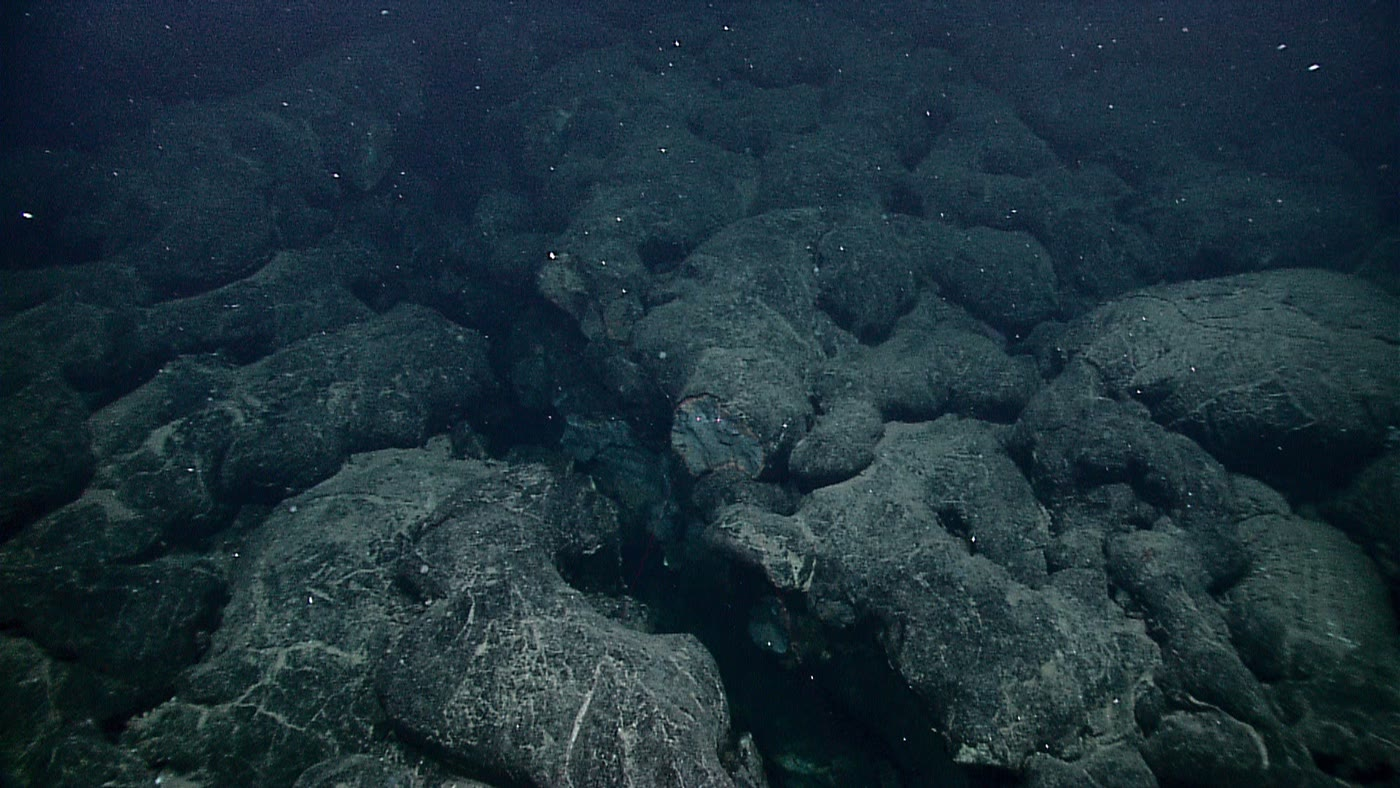
\includegraphics[width=0.6\linewidth]{images/book3/b1-pillow-lava.jpg}

{\small \omterm{def:b1:rifts-ridges-margins:oceanic-crust}{Kussenlava}'s op de Galápagos-rift, doorsneden door een spleet die openging nadat zij waren gestold: de bovenkant van laag~2 van de \omterm{def:b1:rifts-ridges-margins:oceanic-crust}{oceanische korst} terwijl zij ontstaat. Elke kussen is een tong van lava die van buitenaf door het zeewater is bevroren. Foto: NOAA Okeanos Explorer Program, Galápagos Rift Expedition 2011, CC~BY~2.0 (Wikimedia Commons).}
\label{fig:b1:rifts-ridges-margins:pillows}
\end{omfigure}
% ledger: commons:pillow-expl6453

\begin{proposition}[Elke gang splijt de vorige]\label{prop:b1:rifts-ridges-margins:dykes}
Veronderstel dat elke gang van een \omterm{def:b1:rifts-ridges-margins:oceanic-crust}{gangencomplex van platen} langs de spreidingsas wordt geïntrudeerd, waar de \omterm{def:b1:layered-earth:layers}{korst} het heetst en het zwakst is, en dat de \omterm{def:b1:layered-earth:layers}{korst} symmetrisch van de as wegbeweegt. Dan worden de meeste gangen in tweeën gesplitst gevonden, elke helft met een gestolde rand alleen tegen haar oudere buur.
\end{proposition}

\begin{proof}
Een gang koelt af tegen het koudere gesteente aan beide kanten: zij heeft twee gestolde randen wanneer zij ontstaat. De volgende gang stijgt op waar de \omterm{def:b1:layered-earth:layers}{korst} het zwakst is, langs de as, dat wil zeggen door het midden van de vorige, nog steeds het heetste gesteente. Zij splitst die in twee helften, die de spreiding naar weerszijden wegvoert; elke helft houdt de gestolde rand aan haar buitenkant en heeft aan haar binnenkant het niet-afgekoelde contact met de nieuwe gang. Elke gang behalve de laatste wordt zo gesplitst.
\end{proof}

Gangen met een gestolde rand aan slechts één kant zijn inderdaad de regel in gangencomplexen: het kenmerk van een \omterm{def:b1:layered-earth:layers}{korst} die gang na gang door spreiding is opgebouwd.


\section{De diepte--leeftijdswet}\label{sec:b1:rifts-ridges-margins:depth-age}

De oceaanbodem is ondiep bij de rug en diep ver ervandaan. Omdat de bodem bij de rug wordt gemaakt en weggevoerd, is de afstand tot de rug de leeftijd, en hangt de diepte van de bodem van haar leeftijd af. De plaat koelt van boven af terwijl zij ouder wordt (\cref{ch:b1:heat-budget}); koud gesteente is dichter, en een dichtere kolom drijft lager.

\begin{lemma}[Een integraal van de foutenfunctie]\label{lem:b1:rifts-ridges-margins:erfc}
Met $\operatorname{erfc} u = 1 - \operatorname{erf} u =
\frac{2}{\sqrt\pi}\int_u^\infty e^{-s^2}\,\mathrm ds$,
\[
  \int_0^\infty \operatorname{erfc} u \,\mathrm du = \frac{1}{\sqrt\pi}.
\]
\end{lemma}

\begin{proof}
De afgeleide van $\operatorname{erfc}$ is $-\frac{2}{\sqrt\pi}e^{-u^2}$.
Door partieel te integreren op $[0, X]$,
\[
  \int_0^X \operatorname{erfc} u\,\mathrm du
  = \bigl[u \operatorname{erfc} u\bigr]_0^X + \frac{2}{\sqrt\pi}\int_0^X u\,e^{-u^2}\,\mathrm du
  = X\operatorname{erfc} X + \frac{1}{\sqrt\pi}\bigl(1 - e^{-X^2}\bigr).
\]
Voor $X > 0$ en $s \ge X$ geldt $e^{-s^2} \le (s/X)e^{-s^2}$, dus
$X\operatorname{erfc} X \le \frac{2}{\sqrt\pi}\int_X^\infty s\,e^{-s^2}\,\mathrm ds
= e^{-X^2}/\sqrt\pi$, wat naar 0 gaat. Als $X \to \infty$ gaat, volgt het resultaat.
\end{proof}

\begin{theorem}[Diepte--leeftijdswet]\label{thm:b1:rifts-ridges-margins:depth-age}
Neem aan dat
\begin{enumerate}
  \item de \omterm{def:b1:layered-earth:layers}{mantel} de rug verlaat op de uniforme temperatuur $T_m$, en de oceanische plaat van leeftijd $t$ een halfruimte is die sindsdien vanaf haar oppervlak is afgekoeld, op $T_0$ gehouden, met de thermische diffusiviteit $\kappa$;
  \item de dichtheid van het afgekoelde gesteente $\rho_m\bigl(1 + \alpha(T_m -
        T)\bigr)$ is, met $\rho_m$ de dichtheid van de \omterm{def:b1:layered-earth:layers}{mantel} bij $T_m$ en
        $\alpha$ haar uitzettingscoëfficiënt;
  \item elke kolom in isostatisch evenwicht is boven een \omterm{def:b1:isostasy-gravity:isostasy}{compensatiediepte} die onder de afgekoelde laag ligt, en zeewater de dichtheid $\rho_w$ heeft.
\end{enumerate}
Dan wordt de diepte van de zeebodem van leeftijd $t$ gegeven door
\[
  d(t) = d_r + C\sqrt t, \qquad
  C = \frac{2}{\sqrt\pi}\,\frac{\rho_m\,\alpha\,(T_m - T_0)\sqrt\kappa}{\rho_m - \rho_w},
\]
waarin $d_r$ de diepte van de rugas is. Dit is de \emph{diepte--leeftijdswet}\index{diepte--leeftijdswet} van de oceaanbodem.
\end{theorem}

\begin{proof}
De temperatuur in de afgekoelde halfruimte is
\[
  T(z, t) = T_0 + (T_m - T_0)\operatorname{erf}\frac{z}{2\sqrt{\kappa t}},
\]
met $z$ de diepte onder de zeebodem; deze oplossing van de warmtevergelijking wordt hier aangenomen, zoals in \cref{ch:b1:heat-budget}, en in Boek 5 afgeleid. Vergelijk de kolom bij de rug, die uit water tot $d_r$ bestaat en daaronder uit \omterm{def:b1:layered-earth:layers}{mantel} op $T_m$, met de kolom van leeftijd $t$, die uit water tot $d$ bestaat en daaronder uit de afgekoelde plaat, beide tot de \omterm{def:b1:isostasy-gravity:isostasy}{compensatiediepte} $D$. Hun massa's per oppervlakte-eenheid zijn gelijk:
\[
  \rho_w d_r + \rho_m (D - d_r) = \rho_w d + \int_0^{D-d}\rho_m\bigl(1 + \alpha(T_m - T)\bigr)\mathrm dz
  = \rho_w d + \rho_m (D - d) + \rho_m\alpha\int_0^{D-d}(T_m - T)\,\mathrm dz.
\]
Dus
\[
  (\rho_m - \rho_w)(d - d_r) = \rho_m\alpha\int_0^{D-d}(T_m - T)\,\mathrm dz.
\]
Omdat $T_m - T = (T_m - T_0)\operatorname{erfc}\bigl(z/2\sqrt{\kappa t}\bigr)$ onder de afgekoelde laag verwaarloosbaar is, mag de integraal tot oneindig worden genomen; met $u = z/2\sqrt{\kappa t}$ en \cref{lem:b1:rifts-ridges-margins:erfc},
\[
  \int_0^\infty (T_m - T)\,\mathrm dz = (T_m - T_0)\,2\sqrt{\kappa t}\int_0^\infty\operatorname{erfc}u\,\mathrm du
  = \frac{2}{\sqrt\pi}(T_m - T_0)\sqrt{\kappa t}.
\]
Delen door $\rho_m - \rho_w$ geeft $d - d_r = C\sqrt t$.
\end{proof}

Het water telt mee: naarmate de plaat zinkt, vult water de ruimte erboven, en het gewicht daarvan drukt de plaat verder naar beneden. De effectieve uitzettingscoëfficiënt $\alpha\rho_m/(\rho_m - \rho_w)$ is groter dan $\alpha$ met de factor $3300/2300 \approx 1.43$.

Met $\alpha = \qty{3.2e-5}{K^{-1}}$, $T_m - T_0 = \qty{1350}{K}$, $\kappa = \qty{e-6}{m^2.s^{-1}}$, $\rho_m = \qty{3300}{kg.m^{-3}}$ en $\rho_w = \qty{1000}{kg.m^{-3}}$, en de tijd uitgedrukt in miljoenen jaren ($\sqrt{\kappa\times\qty{1}{Myr}} = \qty{5618}{m}$), geeft de stelling $C = \qty{393}{m.Myr^{-1/2}}$. De constanten die Parsons en Sclater aan de diepten van de Noord-Pacifische en de Noord-Atlantische Oceaan hebben gepast, nadat de sedimenten zijn verwijderd, komen dicht in de buurt: $d_r \approx \qty{2500}{m}$ en $C \approx \qty{350}{m.Myr^{-1/2}}$, van 0 tot \qty{70}{Myr}. De waarden van $\alpha$ en $T_m$ die hierboven zijn gebruikt, zijn die van hun plaatmodel voor oude bodem, een \omterm{def:b1:layered-earth:layers}{mantel} op \qty{1350}{\degreeCelsius} en $\alpha = \qty{3.2e-5}{\per\degreeCelsius}$, onzeker met respectievelijk een vijfde en een derde, zodat de overeenstemming van 393 met 350 zo goed is als men kon hopen.
% ledger: parsons:plate-model, ps77:depth-age

\begin{example}[Oceaanbodem van 25 en 100 miljoen jaar oud]\label{ex:b1:rifts-ridges-margins:depths}
Met $d = 2500 + 350\sqrt t$ (meter, $t$ in miljoenen jaren) ligt bodem van \qty{25}{Myr} oud op $2500 + 350\times5 = \qty{4250}{m}$ en bodem van \qty{100}{Myr} oud op $2500 + 350\times10 = \qty{6000}{m}$. De bodem zakt \qty{1750}{m} in haar eerste 25 miljoen jaar, en nog slechts \qty{1750}{m} in de volgende 75.
\end{example}
% ledger: parsons:plate-model

\begin{omfigure}
\begin{tikzpicture}
\begin{axis}[omrecord, omdepth, width=0.84\linewidth, height=6.6cm,
  xmin=0, xmax=13.6, ymin=2000, ymax=6800,
  xlabel={vierkantswortel van de leeftijd van de bodem, $\sqrt t$ (\unit{Myr^{1/2}})},
  ylabel={diepte (\unit{m})},
  yticklabel style={/pgf/number format/set thousands separator={}},
  legend style={font=\scriptsize, at={(0.02,0.03)}, anchor=south west, draw=none, fill=white, fill opacity=0.85, text opacity=1},
  legend cell align=left]
% computed in figdata/bachelor-1/depth_age.py; ledger: data:etopo1, data:b2-seafloor-age, parsons:plate-model
\addplot[name path=lo, draw=none, forget plot] table[x expr=sqrt(\thisrow{t}), y=q1] {figdata/out/bachelor-1-depth_age-bins.dat};
\addplot[name path=hi, draw=none, forget plot] table[x expr=sqrt(\thisrow{t}), y=q3] {figdata/out/bachelor-1-depth_age-bins.dat};
\addplot[black!12] fill between[of=lo and hi];
\addlegendentry{middelste helft van de cellen}
\addplot[only marks, mark=*, mark size=1.1pt, black!70] table[x expr=sqrt(\thisrow{t}), y=median] {figdata/out/bachelor-1-depth_age-bins.dat};
\addlegendentry{mediane diepte, leeftijdsklassen van 2-Myr}
\addplot[very thick, omProp] table[x expr=sqrt(\thisrow{t}), y=halfspace] {figdata/out/bachelor-1-depth_age-models.dat};
\addlegendentry{halfruimte, $2500 + 350\sqrt t$}
\addplot[thick, omDef, densely dashed] table[x expr=sqrt(\thisrow{t}), y=plate] {figdata/out/bachelor-1-depth_age-models.dat};
\addlegendentry{plaatmodel, $6400 - 3200\,e^{-t/62.8}$}
\draw[black!50, densely dotted] (axis cs:8.944,2000) -- (axis cs:8.944,6800);
\node[font=\scriptsize, anchor=north west, black!70] at (axis cs:8.944,2060) {\qty{80}{Myr}};
\node[font=\scriptsize, anchor=north west, black!70] at (axis cs:4.472,2060) {\qty{20}{Myr}};
\draw[black!50, densely dotted] (axis cs:4.472,2000) -- (axis cs:4.472,6800);
\end{axis}
\end{tikzpicture}

{\small Diepte van de oceaanbodem tegen de vierkantswortel van haar leeftijd. Elk punt is de mediane diepte van de cellen van één graad van de wereldoceaan waarvan de bodem in een leeftijdsklasse van twee miljoen jaar valt (31\,538 cellen, dieper dan \qty{1000}{m}); de grijze band bevat de middelste helft ervan. De wet van de halfruimte is in deze grafiek een rechte lijn. Jonge bodem volgt haar nauwkeurig; oudere bodem ligt erboven, omdat de cellen hun sedimenten meenemen en zeebergen en vulkanische plateaus omvatten, en omdat oude bodem ophoudt te zinken (gestippeld: het plaatmodel). Gegevens: ETOPO1 (NOAA) en de leeftijden van de oceaanbodem van Seton en anderen (2020).}
\label{fig:b1:rifts-ridges-margins:depth-age}
\end{omfigure}

De figuur toetst de stelling aan de hele oceaan. Tot ongeveer \qty{20}{Myr} ($\sqrt t \approx 4.5$) liggen de medianen binnen ongeveer honderd meter van de wet. Een rechte lijn die door de medianen jonger dan \qty{70}{Myr} is gepast, heeft een helling van slechts \qty{250}{m.Myr^{-1/2}}: de gemeten diepten zijn die van het sedimentoppervlak, terwijl de wet de diepte van de bovenkant van de \omterm{def:b1:layered-earth:layers}{korst} geeft, en de sedimentdeklaag dikt met de leeftijd aan. Tussen 60 en \qty{80}{Myr} wijkt de bodem af van de wet van de vierkantswortel, zelfs nadat de sedimenten zijn verwijderd: zij wordt ondieper dan de wet en houdt op met zinken. Het plaatmodel, een plaat van \qty{125}{km} dik waarvan de basis op de mantel-temperatuur wordt gehouden, beschrijft deze afvlakking: haar diepte nadert ongeveer \qty{6400}{m}, en haar \omterm{def:b1:heat-budget:heat-flow}{warmtestroom} een constante, alsof warmte aan de basis van oude platen door de convecterende \omterm{def:b1:layered-earth:layers}{mantel} wordt toegevoerd. Dat model wordt bestudeerd in Boek 5; in dit boek wordt de wet van de vierkantswortel tot \qty{80}{Myr} gebruikt.
% ledger: parsons:plate-model; fit and cell count from depth_age.py (values part)

\begin{method}[Oceaanbodem dateren uit haar diepte]\label{met:b1:rifts-ridges-margins:age-from-depth}
Om de leeftijd van oceaanbodem te schatten waar haar magnetische anomalieën ontbreken of niet in kaart zijn gebracht:
\begin{enumerate}
  \item meet de diepte van de bodem en, uit seismische profielen, de dikte van haar sedimenten; neem de diepte $d$ van de bovenkant van de \omterm{def:b1:layered-earth:layers}{korst}, gecorrigeerd voor het gewicht van de sedimenten;
  \item inverteer de wet: $t = \bigl((d - d_r)/C\bigr)^2$, met $d_r$ en $C$ voor de betrokken oceaan;
  \item controleer dat de bodem jonger is dan ongeveer \qty{80}{Myr}, en schat de onzekerheid: een fout $\delta d$ in de diepte geeft $\delta t = 2t\,\delta d/(d - d_r)$.
\end{enumerate}
\end{method}

Voor bodem op \qty{4600}{m} geldt $t = (2100/350)^2 = \qty{36}{Myr}$, en een onzekerheid van \qty{100}{m} in de diepte geeft $2\times36\times100/2100 \approx
\qty{3.4}{Myr}$ op de leeftijd. Waar bodem over een breed gebied ondieper ligt dan de wet voorspelt, een zwelling, is de oorzaak geen leeftijd maar warmte van onderaf (\cref{ch:b1:hotspots}).

De wet verbindt de oceaan ook met de zeespiegel. Een rug die sneller spreidt voert jonge, ondiepe bodem verder van haar as weg; de oceaanbekkens bevatten dan minder water, en de zee stijgt over de continenten. Over tientallen miljoenen jaren zijn veranderingen in de spreidingssnelheid één van de twee belangrijkste oorzaken van de veranderingen van de mondiale zeespiegel, naast het volume van het land-ijs.

\section{Transformbreuken en breukzones}

Ruggen zijn geen doorlopende lijnen: zij zijn in segmenten gesneden, verschoven door breuken die loodrecht op hen lopen, langs de richting van de spreiding. Voorbij de verschuivingen zetten de breuken zich voort als lange littekens over de oceaanbodem.

\begin{definition}[Transformbreuk, breukzone]\label{def:b1:rifts-ridges-margins:transform}
Een \emph{transformbreuk}\index{transformbreuk} is een horizontale verschuivingsbreuk die een plaatgrens is en eindigt bij andere plaatgrenzen; een transform tussen twee ruggen verbindt de uiteinden van twee verschoven ruggensegmenten. Een \emph{breukzone}\index{breukzone} is de voortzetting van een transformbreuk voorbij de uiteinden van de ruggensegmenten: een lineaire vallei of trap over de oceaanbodem die bodem van verschillende leeftijd scheidt en tot één plaat behoort.
\end{definition}

\begin{proposition}[Verschuiving op een transform tussen twee ruggen]\label{prop:b1:rifts-ridges-margins:transform}
Twee ruggensegmenten die symmetrisch spreiden met de halve snelheid $u$, loodrecht op zichzelf, zijn verschoven door een \omterm{def:b1:rifts-ridges-margins:transform}{transformbreuk} van lengte $a$. Dan:
\begin{enumerate}
  \item de twee zijden van de transform schuiven langs elkaar met de volle snelheid $2u$, in de zin tegengesteld aan die welke de verschuiving zou suggereren als één rechte rug was doorgesneden en door de breuk was verplaatst;
  \item langs de \omterm{def:b1:rifts-ridges-margins:transform}{breukzones} bewegen de twee zijden niet ten opzichte van elkaar, en verschilt de bodem aan beide zijden in leeftijd met $a/u$;
  \item de lengte van de transform verandert niet met de tijd.
\end{enumerate}
\end{proposition}

\begin{proof}
Neem de $x$-as langs de transform, naar het oosten, en de $y$-as naar het noorden, in het stelsel van de rug. Laat het noordelijke segment op $x = 0$, $y > 0$ liggen, en het zuidelijke op $x = a$, $y < 0$ (de verschuiving gaat naar het oosten richting zuid); de transform is het segment $0 < x < a$ van $y = 0$. De westelijke plaat $W$ ligt ten westen van beide segmenten en beweegt met $-u$ langs $x$; de oostelijke plaat $E$ ligt ten oosten van beide en beweegt met $+u$.

(1) Net ten noorden van de transform, bij $0 < x < a$, ligt de bodem ten oosten van het noordelijke segment: zij hoort bij $E$ en beweegt naar het oosten met $u$. Net ten zuiden ervan ligt de bodem ten westen van het zuidelijke segment: zij hoort bij $W$ en beweegt naar het westen met $u$. De noordelijke zijde beweegt naar het oosten met $2u$ ten opzichte van de zuidelijke zijde: gezien vanaf beide zijden gaat de verre zijde naar rechts, en de verschuiving is rechtszijdig (dextraal). Een rechte rug, door de breuk doorgesneden, waarvan het zuidelijke deel nu ten oosten van het noordelijke deel ligt, zou daarentegen een linkszijdige (sinistrale) verplaatsing hebben vastgelegd.

(2) Voor $x > a$ liggen beide zijden ten oosten van hun segmenten en horen zij bij $E$: zij bewegen samen. Op de afstand $x$ van het noordelijke segment heeft bodem ten noorden van de \omterm{def:b1:rifts-ridges-margins:transform}{breukzone} de leeftijd $x/u$; bodem ten zuiden ervan ligt op $x - a$ van het zuidelijke segment en heeft de leeftijd $(x - a)/u$. Het verschil is $a/u$. Hetzelfde geldt voor $x < 0$, waar beide zijden bij $W$ horen.

(3) Beide segmenten blijven op $x = 0$ en $x = a$ in het stelsel van de rug, omdat elk symmetrisch spreidt: de transform behoudt de lengte $a$.
\end{proof}

J.\ Tuzo Wilson zag in 1965 dat verschuivingen van ruggen niet kunnen worden gelezen als de verplaatsing van een oudere, rechte rug, en voorspelde de zin van de verschuiving uit de propositie; de focale mechanismen van aardbevingen op transforms bevestigden dat. Aardbevingen komen voor langs de actieve transform, tussen de uiteinden van de ruggen; de \omterm{def:b1:rifts-ridges-margins:transform}{breukzones} zijn meestal stil. Over een \omterm{def:b1:rifts-ridges-margins:transform}{breukzone} heen hebben de bodem van de twee zijden verschillende leeftijden, en dus, volgens de \omterm{thm:b1:rifts-ridges-margins:depth-age}{diepte--leeftijdswet}, verschillende diepten: een trap die langzaam vervaagt met de afstand tot de rug. In de Noord-Atlantische Oceaan nabij \ang{52}\,N verschuiven de twee Charlie--Gibbs-transforms de Mid-Atlantische Rug samen over ongeveer \qty{350}{km}.
% ledger: wilson:transform, data:pb2002 (offset summed over the transform steps in figdata/bachelor-1/ridge_budget.py)

\begin{omfigure}
\begin{tikzpicture}[x=0.95cm, y=0.95cm, font=\scriptsize]
\fill[omSea!10] (-5,-2.6) rectangle (8,2.6);
% isochrons (10 and 20 Myr), offset across the fracture zones
\foreach \x in {-4,-2,2,4} \draw[black!40] (\x,0) -- (\x,2.5);
\foreach \x in {-1,1,5,7} \draw[black!40] (\x,0) -- (\x,-2.5);
\node[black!55, anchor=south, fill=omSea!10, inner sep=1pt] at (2,2.0) {10};
\node[black!55, anchor=south, fill=omSea!10, inner sep=1pt] at (4,2.0) {20};
\node[black!55, anchor=south, fill=omSea!10, inner sep=1pt] at (-2,2.0) {10};
\node[black!55, anchor=south, fill=omSea!10, inner sep=1pt] at (-4,2.0) {20};
\node[black!55, anchor=north, fill=omSea!10, inner sep=1pt] at (5,-2.0) {10};
\node[black!55, anchor=north, fill=omSea!10, inner sep=1pt] at (7,-2.0) {20};
\node[black!55, anchor=north, fill=omSea!10, inner sep=1pt] at (1,-2.0) {10};
\node[black!55, anchor=north, fill=omSea!10, inner sep=1pt] at (-1,-2.0) {20};
% fracture zones and transform
\draw[black!60, thick, densely dashed] (-5,0) -- (0,0);
\draw[black!60, thick, densely dashed] (3,0) -- (8,0);
\draw[transform, line width=1.4pt] (0,0) -- (3,0);
% ridge segments
\draw[ridge, line width=1.1pt] (0,0) -- (0,2.6);
\draw[ridge, line width=1.1pt] (3,0) -- (3,-2.6);
\pic at (1.5,0) {dextral={90}};
\foreach \x in {0.4,0.75,2.25,2.6} \node[star, star points=5, star point ratio=2.2, fill=orange!90!black, draw=black, line width=0.2pt, inner sep=1.5pt] at (\x,0.0) {};
% plate motions
\draw[-{Stealth[length=4pt]}, very thick, black!70] (-2.8,1.1) -- (-3.9,1.1);
\draw[-{Stealth[length=4pt]}, very thick, black!70] (-0.2,-1.1) -- (-1.3,-1.1);
\draw[-{Stealth[length=4pt]}, very thick, black!70] (5.5,1.1) -- (6.6,1.1);
\draw[-{Stealth[length=4pt]}, very thick, black!70] (5.3,-1.1) -- (6.4,-1.1);
\node[font=\small] at (-3.3,1.55) {plaat $W$};
\node[font=\small] at (6.1,1.55) {plaat $E$};
\node[anchor=west, omRidge] at (0.1,2.25) {rug};
\node[anchor=east, omRidge] at (2.9,-2.25) {rug};
\node[anchor=north, align=center, fill=white, fill opacity=0.8, text opacity=1, inner sep=1pt] at (1.5,-0.35) {transformbreuk\\(actief, aardbevingen)};
\node[anchor=south, fill=white, fill opacity=0.8, text opacity=1, inner sep=1pt] at (5.5,0.12) {breukzone (inactief)};
\node[anchor=north, fill=white, fill opacity=0.8, text opacity=1, inner sep=1pt] at (-2.5,-0.12) {breukzone (inactief)};
\node[anchor=south, black!70, fill=omSea!10, inner sep=1pt] at (6.2,0.55) {ouder, dieper};
\node[anchor=north, black!70, fill=omSea!10, inner sep=1pt] at (6.0,-0.45) {jonger, ondieper};
\end{tikzpicture}

{\small Een rugsegment dat door een \omterm{def:b1:rifts-ridges-margins:transform}{transformbreuk} is verschoven, in kaartbeeld, het noorden boven. De twee platen bewegen van elk segment weg (zwarte pijlen); langs de transform (rood) schuiven zij rechtszijdig langs elkaar (halve pijlen), hoewel de verschuiving van de rug linkszijdig lijkt. Grijze lijnen zijn isochronen, met de leeftijd in miljoenen jaren; over elke \omterm{def:b1:rifts-ridges-margins:transform}{breukzone} (gestippeld) ligt bodem van verschillende leeftijd, dus van verschillende diepte, naast elkaar, maar beide zijden bewegen samen. Sterren: aardbevingen, beperkt tot de transform.}
\label{fig:b1:rifts-ridges-margins:transform}
\end{omfigure}

Transforms zijn het derde bewijs voor de plaatbewegingen van \cref{ch:b1:plate-kinematics}: een transform loopt langs de relatieve snelheid van de twee platen, dus ligt hij op een \omterm{def:b1:spherical-astronomy:spherical-triangle}{kleine cirkel} om hun \omterm{def:b1:plate-kinematics:euler-pole}{Eulerpool}, en de grote cirkels die loodrecht op verschillende transforms worden getekend, snijden elkaar in de pool. \omterm{def:b1:rifts-ridges-margins:transform}{Breukzones}, over de oceaanbodem getraceerd, leggen de bewegingsrichting uit het verleden vast, zoals de magnetische anomalieën de snelheid vastleggen.

\section{Oefeningen}

\begin{exercise}[$\star$]\label{exo:b1:rifts-ridges-margins:1}
In 2005 opende zich een segment van het Afar-rift, \qty{60}{km} lang, tot \qty{8}{m}, en werd \qty{2.5}{km^3} magma geïntrudeerd. (a) Als de gang over het hele segment \qty{8}{m} dik was geweest, hoe groot zou haar gemiddelde hoogte dan zijn geweest? (b) Hoeveel jaar beweging vertegenwoordigt een opening van \qty{8}{m} bij de plaatsnelheid van \qty{18}{mm.yr^{-1}}?
% ledger: wright:afar, morvel:ar-nb
\end{exercise}

\begin{exercise}[$\star$]\label{exo:b1:rifts-ridges-margins:2}
Een \omterm{def:b1:rifts-ridges-margins:rift}{halve slenk} wordt begrensd door een randbreuk met \omterm{def:b1:cross-sections:throw}{worp} \qty{3.0}{km} en helling \ang{60}, en doorsneden door een kleinere antithetische breuk met \omterm{def:b1:cross-sections:throw}{worp} \qty{0.8}{km} en helling \ang{70}. (a) Bereken de \omterm{def:b1:cross-sections:throw}{heave} van elke breuk en de uitrekking van de doorsnede. (b) De doorsnede is nu \qty{25}{km} breed: hoe breed was zij voor de breuken ontstonden?
\end{exercise}

\begin{exercise}[$\star$]\label{exo:b1:rifts-ridges-margins:3}
Rangschik de volgende ruggen met de grenzen van de definitie, uit hun volledige spreidingssnelheden berekend met plaatvectoren: Gakkelrug \qty{12}{mm.yr^{-1}}; centrale Rode Zee \qty{15}{mm.yr^{-1}}; Reykjanes-rug \qty{19}{mm.yr^{-1}}; westelijke Carlsbergrug \qty{23}{mm.yr^{-1}}; Zuid-Atlantische Oceaan bij \ang{20}\,S \qty{33}{mm.yr^{-1}}; Oost-Pacifische Rug bij \ang{20}\,S \qty{143}{mm.yr^{-1}}. Welke daarvan verwacht men met een as-dal te vinden, en welke met een as-hoogte?
% ledger: morvel:eu-na, morvel:redsea, morvel:in-sm, morvel:nb-sa, morvel:nz-pa (rates computed with euler_velocities.py)
\end{exercise}

\begin{exercise}[$\star$]\label{exo:b1:rifts-ridges-margins:4}
Ongeveer \qty{3.0}{km^2} nieuwe oceaanbodem wordt elk jaar gemaakt, met een \omterm{def:b1:layered-earth:layers}{korst} van \qty{7.1}{km} dik. (a) Welk volume \omterm{def:b1:layered-earth:layers}{korst} wordt elk jaar gemaakt? (b) Hoe lang zou het bij dit tempo duren om de \qty{3.028e8}{km^2} oceaanbodem te maken? Vergelijk met de leeftijd van de oudste oceaanbodem, ongeveer \qty{190}{Myr}, en leg uit waarom de twee niet hoeven overeen te komen.
% ledger: data:pb2002 (ridge_budget.py), white:crust, dd10:split, data:b2-seafloor-age
\end{exercise}

\begin{exercise}[$\star\star$]\label{exo:b1:rifts-ridges-margins:5}
Met $d = 2500 + 350\sqrt t$ (meter, $t$ in miljoenen jaren): (a) bereken de diepte van bodem van 4, 36 en 64 miljoen jaar oud; (b) zoek de leeftijd van bodem die op \qty{4600}{m} en op \qty{5300}{m} ligt; (c) hoeveel zinkt de bodem tussen 4 en \qty{36}{Myr}, en tussen 36 en \qty{64}{Myr}?
\end{exercise}

\begin{exercise}[$\star\star$]\label{exo:b1:rifts-ridges-margins:6}
Bereken de constante $C$ van de \omterm{thm:b1:rifts-ridges-margins:depth-age}{diepte--leeftijdswet} (\cref{thm:b1:rifts-ridges-margins:depth-age}) voor $\alpha =
\qty{3.2e-5}{K^{-1}}$, $\rho_m = \qty{3300}{kg.m^{-3}}$, $\rho_w =
\qty{1000}{kg.m^{-3}}$, $T_m - T_0 = \qty{1350}{K}$ en $\kappa =
\qty{e-6}{m^2.s^{-1}}$, in \unit{m.Myr^{-1/2}}. Herhaal dit voor een \omterm{def:b1:layered-earth:layers}{mantel} die \qty{250}{K} kouder is. Welke constante zou de bodem van een koudere oceaan volgen?
% ledger: parsons:plate-model
\end{exercise}

\begin{exercise}[$\star\star$]\label{exo:b1:rifts-ridges-margins:7}
Het plaatmodel geeft de \omterm{def:b1:heat-budget:heat-flow}{warmtestroom} van de oceaanbodem als $q = 11.3/\sqrt t$, in eenheden van \qty{e-6}{cal.cm^{-2}.s^{-1}}, met $t$ in miljoenen jaren. (a) Reken de constante om naar \unit{mW.m^{-2}.Myr^{1/2}} ($\qty{1}{cal} =
\qty{4.184}{J}$) en vergelijk haar met de \qty{490}{mW.m^{-2}.Myr^{1/2}} van
\cref{ch:b1:heat-budget}. (b) Bereken $q$ bij 1, 10 en \qty{150}{Myr}. De wet werd gepast aan bodem tot \qty{120}{Myr} oud, en het plaatmodel laat de \omterm{def:b1:heat-budget:heat-flow}{warmtestroom} van oudere bodem tot een constante afvlakken: is de waarde bij \qty{150}{Myr} dan te hoog of te laag?
% ledger: parsons:plate-model, dd10:young-ocean
\end{exercise}

\begin{exercise}[$\star\star$]\label{exo:b1:rifts-ridges-margins:8}
Een rug die noord--zuid loopt, is in twee segmenten gesneden; gaat men langs de rug naar het zuiden, dan springt de as bij een \omterm{def:b1:rifts-ridges-margins:transform}{transformbreuk} \qty{40}{km} naar het \emph{westen}. (a) Wat is de zin van de verschuiving op de transform? (b) Wat lijkt de verschuiving van de rug aan te tonen? (c) Waar langs de lijn van de transform komen aardbevingen voor, en waarom niet verder?
\end{exercise}

\begin{exercise}[$\star\star$]\label{exo:b1:rifts-ridges-margins:9}
De \omterm{def:b1:rifts-ridges-margins:transform}{breukzones} van Charlie--Gibbs verschuiven de Mid-Atlantische Rug samen over \qty{350}{km}; de volledige spreidingssnelheid is daar \qty{21.2}{mm.yr^{-1}}. Behandel de verschuiving als één transform. (a) Wat is het leeftijdsverschil over de \omterm{def:b1:rifts-ridges-margins:transform}{breukzone}? (b) Bereken met $d = 2500 + 350\sqrt t$ de diepte-sprong over de \omterm{def:b1:rifts-ridges-margins:transform}{breukzone} aan het einde van de transform, en daarna op \qty{100}{km} en \qty{1000}{km} erachter.
% ledger: data:pb2002 (ridge_budget.py), morvel:eu-na (rate at 52.5 N 31.5 W from euler_velocities.py)
\end{exercise}

\begin{exercise}[$\star\star\star$]\label{exo:b1:rifts-ridges-margins:10}
Een oceaanbekken wordt tegen een constant tempo gemaakt en bevat bodem van elke leeftijd van 0 tot $A$, in gelijke oppervlakten. (a) Toon aan dat zijn gemiddelde diepte $d_r +
\frac23C\sqrt A$ is. (b) Met $d_r = \qty{2500}{m}$ en
$C = \qty{350}{m.Myr^{-1/2}}$, vergelijk $A = \qty{180}{Myr}$ en
$A = \qty{120}{Myr}$. (c) Als de spreiding van het bekken versnelt zodat haar oudste bodem \qty{120}{Myr} in plaats van \qty{180}{Myr} is, hoeveel stijgt dan de zeespiegel, met verwaarlozing van het onder water zetten van de continenten maar met inrekening van de belasting van het extra water op de bodem, die zakt met $\rho_w/(\rho_m - \rho_w)$ maal de stijging ($\rho_m = 3300$, $\rho_w = \qty{1000}{kg.m^{-3}}$)?
\end{exercise}

\begin{exercise}[$\star\star\star$]\label{exo:b1:rifts-ridges-margins:11}
In de situatie van \cref{prop:b1:rifts-ridges-margins:transform} is de diepte-sprong over een \omterm{def:b1:rifts-ridges-margins:transform}{breukzone} op de afstand $x > a$ van het verste rugsegment $\Delta d = C\bigl(\sqrt{x/u} - \sqrt{(x - a)/u}\bigr)$. (a) Toon aan dat voor $x \gg a$ geldt $\Delta d \approx Ca/(2\sqrt{ux})$. (b) Met
$C = \qty{350}{m.Myr^{-1/2}}$, $a = \qty{350}{km}$ en
$u = \qty{10.6}{km.Myr^{-1}}$, vergelijk de exacte en de benaderde sprong bij
$x = 450$, 1350 en \qty{3350}{km}. Wanneer is de benadering goed tot
\qty{10}{\percent}?
\end{exercise}

\begin{exercise}[$\star\star\star$]\label{exo:b1:rifts-ridges-margins:12}
Vergelijk de halfruimtewet $d_1(t) = 2500 + 350\sqrt t$ met de plaatwet $d_2(t) = 6400 - 3200\,e^{-t/62.8}$. (a) Bereken $d_2 - d_1$ bij 10, 20, 30 en \qty{40}{Myr}. (b) Toon aan dat de twee wetten bij één leeftijd tussen 20 en \qty{30}{Myr} gelijk zijn, en vind die tot \qty{0.1}{Myr} door bissectie. (c) Vergelijk hun hellingen daar. Waarom mogen de twee wetten bij die leeftijd zonder zichtbare breuk aan elkaar worden gekoppeld?
% ledger: parsons:plate-model
\end{exercise}

\section{Probleem: De geboorte van een oceaan}

\begin{problem}[{Weekendprobleem --- een continent uitgerekt door zijn breuken, een jonge oceaan gemeten aan haar magnetische strepen, en de diepte van haar bodem terwijl zij ouder wordt}]
\label{pb:b1:rifts-ridges-margins:1}
% values: calc/ch13.py (Part I rift section and Part II profile invented for the
% problem; real Euler vector, chron ages and depth--age constants)
% ledger: morvel:sm-an, morvel:nb-an, morvel:ar-nb, morvel:redsea, morvel:outward, iodp:gpts2004, heine:sam-saf, parsons:plate-model, wright:afar
Neem $R = \qty{6371}{km}$. Een oceaan wordt in drie stadia geboren, elk vandaag op een andere plaats te zien: een \omterm{def:b1:rifts-ridges-margins:rift}{continentaal rift}, een jonge oceaan en een oude oceaan.

\medskip
\noindent\textbf{Deel I --- Een rift uitgerekt door zijn breuken.} Een doorsnede over een rift met richting \ang{020} snijdt zes normale breuken, waarvan de \omterm{def:b1:cross-sections:throw}{worpen} en hellingen op seismische profielen zijn gemeten:
\begin{center}
\small
\begin{tabular}{lcccccc}
\hline
breuk & F1 & F2 & F3 & F4 & F5 & F6\\
\omterm{def:b1:cross-sections:throw}{worp} (\unit{m}) & 600 & 1100 & 2400 & 350 & 800 & 1500\\
helling & \ang{60} & \ang{55} & \ang{50} & \ang{65} & \ang{60} & \ang{52}\\
\hline
\end{tabular}
\end{center}
De breuken snijden lava's die op \qty{3.2}{Ma} zijn gedateerd, en het rift is nu \qty{60}{km} breed.
\begin{enumerate}
  \item Bereken de \omterm{def:b1:cross-sections:throw}{heave} van elke breuk. Welke is de randbreuk?
  \item Bereken de uitrekking van de doorsnede en de breedte van het rift vóór de breuken ontstonden.
  \item De twee platen scheiden met \qty{6.0}{mm.yr^{-1}} naar \ang{105}. Bereken de component van deze beweging loodrecht op het rift.
  \item Hoe lang zouden de platen erover doen om de uitrekking van vraag 2 te produceren?
  \item Hoeveel zijn de platen uit elkaar bewogen sinds de lava's zijn uitgestroomd? Welk deel daarvan dragen de breuken?
  \item Geef een suggestie waar de rest van de uitrekking is gebleven. Als zij door gangen zoals die van Afar in 2005 is opgenomen, elk \qty{8}{m} breed, hoeveel zouden er nodig zijn, en hoe vaak?
\end{enumerate}

\medskip
\noindent\textbf{Deel II --- Een jonge oceaan gemeten aan haar strepen.} Een magnetisch profiel over de as van de centrale Rode Zee, op \ang{18.0}\,N, \ang{40.0}\,E, loopt langs de spreidingsrichting. De jonge rand van chron C2An (\qty{2.581}{Ma}) ligt \qty{21.0}{km} noordoost van de as en \qty{20.2}{km} zuidwest ervan; de oude rand van chron C3n (\qty{5.235}{Ma}) ligt op \qty{41.0}{km} en \qty{40.2}{km}. De randen van de anomalieën zijn over beide flanken gemiddeld in totaal \qty{2.2}{km} van de as naar buiten verplaatst.
\begin{enumerate}[resume]
  \item Bereken de volledige spreidingssnelheid uit elke chron, zonder correctie.
  \item Corrigeer elke snelheid voor de verplaatsing naar buiten. Komen de twee overeen?
  \item Toon aan dat de snelheid die uit de afstand tussen de twee chrons op elk flank wordt berekend geen correctie nodig heeft, en bereken haar.
  \item Bereken de halve snelheden op elk flank uit de afstanden tussen de twee chrons. Is de spreiding symmetrisch?
  \item De \omterm{def:b1:plate-kinematics:euler-pole}{Eulerpool} van Arabië ten opzichte van Nubië ligt op \ang{30.9}\,N, \ang{23.6}\,E, met de snelheid \qty{0.403}{\degree\per\Myr}. Bereken de hoekafstand van de pool tot het profiel en de volledige spreidingssnelheid die de plaatvector daar voorspelt.
  \item Bereken in de noordelijke Rode Zee, op \ang{26.0}\,N, \ang{35.0}\,E, de hoekafstand tot de pool en de voorspelde snelheid.
  \item Vergelijk deze snelheden met de gemeten 15 en \qty{9}{mm.yr^{-1}}. Waarom opent de Rode Zee in het zuiden sneller?
\end{enumerate}

\medskip
\noindent\textbf{Deel III --- Richting een Atlantische Oceaan.}
\begin{enumerate}[resume]
  \item Hoe breed is de oceaanbodem die in de centrale Rode Zee is gemaakt sinds de oude rand van C3n, tegen het tempo van vraag 9?
  \item De Zuid-Atlantische Oceaan opende zich bij Recife met ongeveer \qty{5000}{km} in \qty{120.6}{Myr} (\cref{ch:b1:plate-kinematics}). Bereken haar gemiddelde openingssnelheid.
  \item Hoe lang zou een opening van \qty{5000}{km} duren bij het huidige tempo van de centrale Rode Zee? En bij dat van de noordelijke Rode Zee?
  \item De Rode Zee opent om een pool die er dicht bij ligt. Wat betekent dit voor haar vorm naarmate zij zich verbreedt, en voor de tijd die het noordelijke deel nodig heeft om de breedte te bereiken die het centrale deel nu heeft?
  \item Tot welk soort rug behoort de as van de Rode Zee, en welke vorm van as verwacht men?
\end{enumerate}

\medskip
\noindent\textbf{Deel IV --- De bodem zinkt.} Gebruik $d = 2500 + 350\sqrt t$ (meter, $t$ in miljoenen jaren) en, ter vergelijking, de plaatwet $6400 - 3200\,e^{-t/62.8}$.
\begin{enumerate}[resume]
  \item Bereken de diepte van de nieuwe bodem op de leeftijden van 1, 10 en \qty{40}{Myr}.
  \item Op welke leeftijd bereikt de bodem \qty{4000}{m}?
  \item De bodem naast elke \omterm{def:b1:rifts-ridges-margins:passive-margin}{passieve rand} is even oud als de oceaan. Hoeveel zakt zij in de eerste \qty{10}{Myr} na de break-up, en tussen 70 en \qty{80}{Myr}?
  \item Met welk tempo, in meter per miljoen jaar, zakt die bodem wanneer de oceaan \qty{80}{Myr} oud is?
  \item Welke \omterm{def:b1:heat-budget:heat-flow}{warmtestroom} verliest de bodem van vraag 22 dan, met $q = 490/\sqrt t$ in \unit{mW.m^{-2}}?
  \item Bereken de diepte van bodem van \qty{80}{Myr} oud met elk van de twee wetten, en hun verschil. Waarom mogen de twee op deze leeftijd worden vergeleken?
  \item Hoe diep plaatst de wet van de vierkantswortel de zeebodem van de nieuwe oceaan, wanneer zij 80 miljoen jaar oud is, tot op een tiende van een kilometer nauwkeurig?
\end{enumerate}
\end{problem}
